\documentclass[11pt,letterpaper]{article}
\usepackage[utf8]{inputenc}
\usepackage[T1]{fontenc}
\usepackage{lmodern}
\usepackage{textcomp}
\usepackage[spanish,es-noshorthands]{babel}
\usepackage[letterpaper,top=3cm,bottom=2.5cm,left=2.5cm,right=2.5cm,headheight=1.1cm,headsep=0.6cm]{geometry}
\usepackage{graphicx}
\usepackage{float}
\usepackage{fancyhdr}
\usepackage{listings}
\usepackage{xcolor}
\usepackage[colorlinks=true,linkcolor=blue,urlcolor=blue]{hyperref}
\urlstyle{same}

\pagestyle{fancy}
\fancyhf{}
\fancyhead[L]{
\includegraphics[height=0.8cm]{imagenes/logo-usm.png}}
\renewcommand{\headrulewidth}{0.4pt}
\renewcommand{\footrulewidth}{0.4pt}
\fancyfoot[L]{SIG}
\fancyfoot[C]{\textbf{\thepage}}
\fancyfoot[R]{Lorenzo Ruiz}

\lstset{
  basicstyle=\ttfamily\small,
  columns=fullflexible,
  keepspaces=true,
  breaklines=true,
  upquote=true,
  aboveskip=6pt,
  belowskip=4pt,
  literate={á}{{\'a}}1 {é}{{\'e}}1 {í}{{\'i}}1 {ó}{{\'o}}1 {ú}{{\'u}}1 {ñ}{{\~n}}1
           {Á}{{\'A}}1 {É}{{\'E}}1 {Í}{{\'I}}1 {Ó}{{\'O}}1 {Ú}{{\'U}}1 {Ñ}{{\~N}}1
}

\begin{document}

\begin{titlepage}
\thispagestyle{empty}
\noindent
\includegraphics[width=0.39\textwidth]{imagenes/logo-industrias.png}

\vspace*{4.2cm}
\noindent\rule{\textwidth}{0.6pt}
\begin{center}
\vspace{-4pt}
{\Huge\textsc{Laboratorio 4}}\\[2pt]
{\large\textsc{Entregable SQL (1/2): Austral Editores}}
\vspace{-4pt}
\end{center}
\noindent\rule{\textwidth}{0.6pt}

\vspace{2.6cm}
\begin{center}
\textbf{Lorenzo Ruiz}\\
Ingeniería Civil Industrial, 202304619-1, \textit{lflandez@usm.cl}\\
Repositorio: \url{https://github.com/LorenzoRF23/ICN292-Lab4-Ruiz-Lorenzo}
\end{center}

\vfill
\begin{center}
\textsc{noviembre, 2026}\\[0.6cm]
\textsc{Campus Vitacura}
\end{center}
\vspace{1.5cm}
\end{titlepage}

\section*{Consulta 1}
\begin{figure}[H]
\begin{lstlisting}
-- Consulta 1
SELECT nombre, genero
FROM autores
WHERE pais <> 'Chile' OR pais IS NULL
ORDER BY nombre;
\end{lstlisting}
\centering
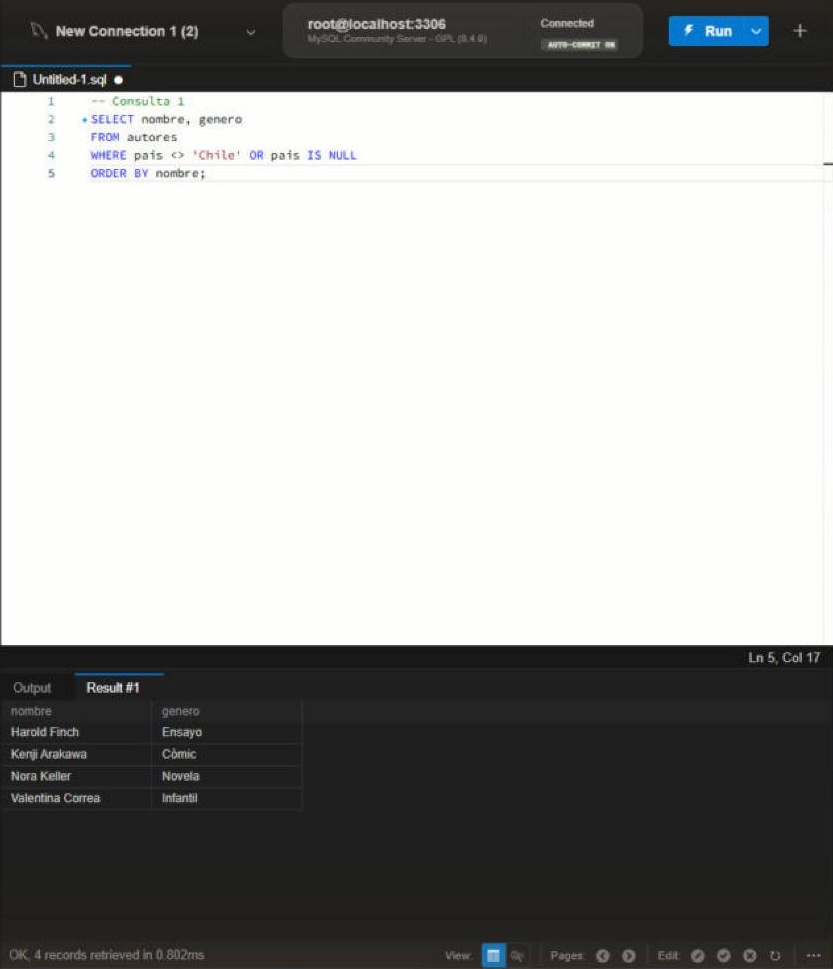
\includegraphics[width=0.72\textwidth]{imagenes/c01.jpg}
\caption{Resultado de la consulta 1}
\end{figure}
\noindent\textbf{Explicación:} \texttt{pais <> \textquotesingle Chile\textquotesingle} da verdadero para los autores de otros países, pero para Kenji Arakawa da NULL, porque cualquier comparación con NULL queda como desconocida; el WHERE descarta esas filas, por eso agregué \texttt{OR pais IS NULL}.

\clearpage
\section*{Consulta 2}
\begin{figure}[H]
\begin{lstlisting}
-- Consulta 2
SELECT titulo, paginas
FROM libros
WHERE paginas >= 190 AND paginas <= 220
ORDER BY paginas ASC;
\end{lstlisting}
\centering
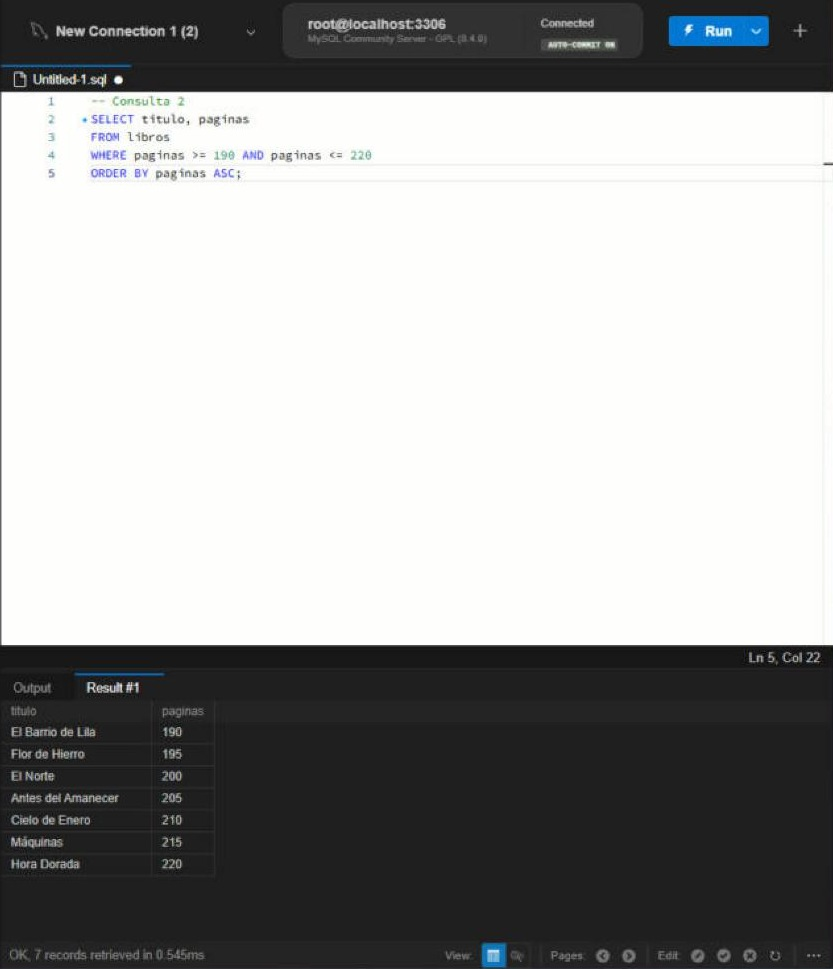
\includegraphics[width=0.72\textwidth]{imagenes/c02.jpg}
\caption{Resultado de la consulta 2}
\end{figure}

\clearpage
\section*{Consulta 3}
\begin{figure}[H]
\begin{lstlisting}
-- Consulta 3
SELECT COUNT(*) AS total_libros,
       SUM(ejemplares_vendidos) AS total_ejemplares_vendidos,
       AVG(paginas) AS promedio_paginas,
       MIN(anio) AS anio_mas_antiguo,
       MAX(ejemplares_vendidos) AS max_ejemplares_un_libro
FROM libros;
\end{lstlisting}
\centering
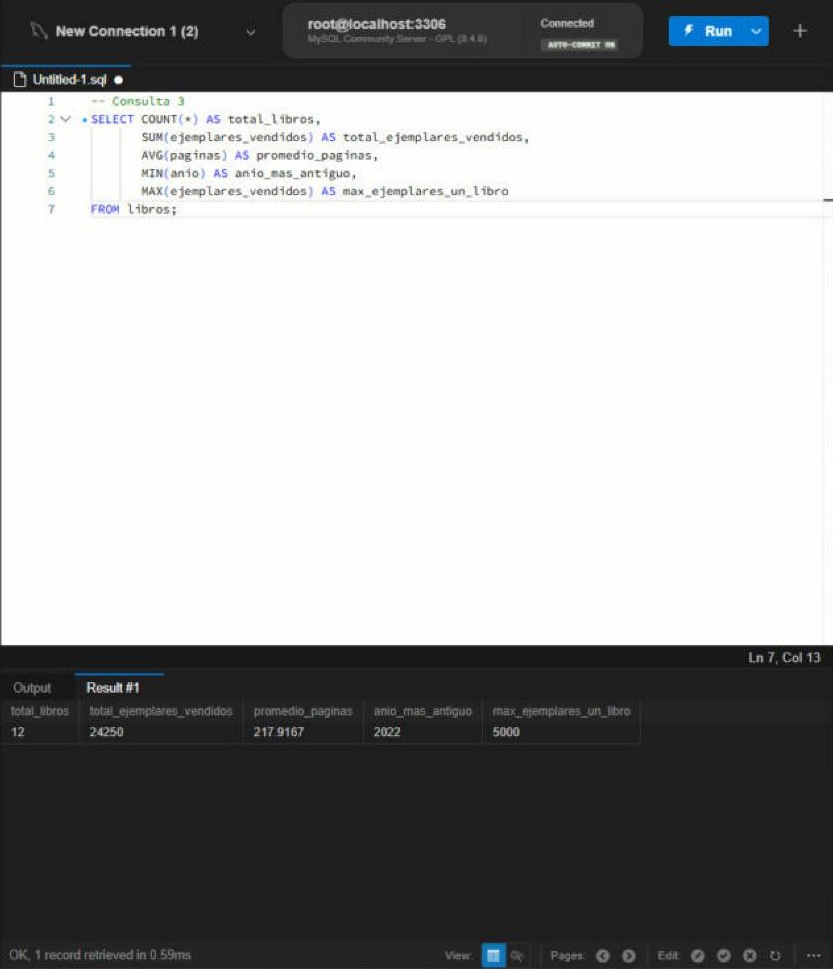
\includegraphics[width=0.72\textwidth]{imagenes/c03.jpg}
\caption{Resultado de la consulta 3}
\end{figure}

\clearpage
\section*{Consulta 4}
\begin{figure}[H]
\begin{lstlisting}
-- Consulta 4
SELECT DISTINCT genero
FROM autores
ORDER BY genero;
\end{lstlisting}
\centering
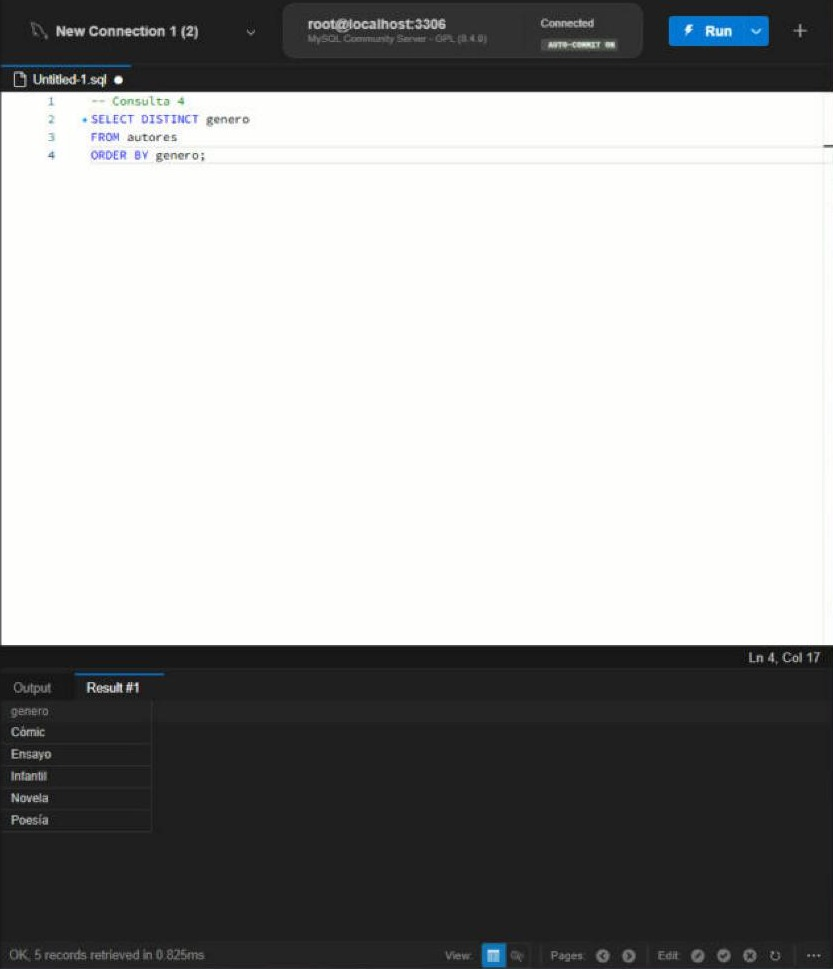
\includegraphics[width=0.72\textwidth]{imagenes/c04.jpg}
\caption{Resultado de la consulta 4}
\end{figure}

\clearpage
\section*{Consulta 5}
\begin{figure}[H]
\begin{lstlisting}
-- Consulta 5
SELECT a.nombre, COUNT(*) AS libros_2024
FROM autores AS a
JOIN libros AS l ON l.id_autor = a.id_autor
WHERE l.anio = 2024
GROUP BY a.id_autor, a.nombre
HAVING COUNT(*) > 1
ORDER BY a.nombre;
\end{lstlisting}
\centering
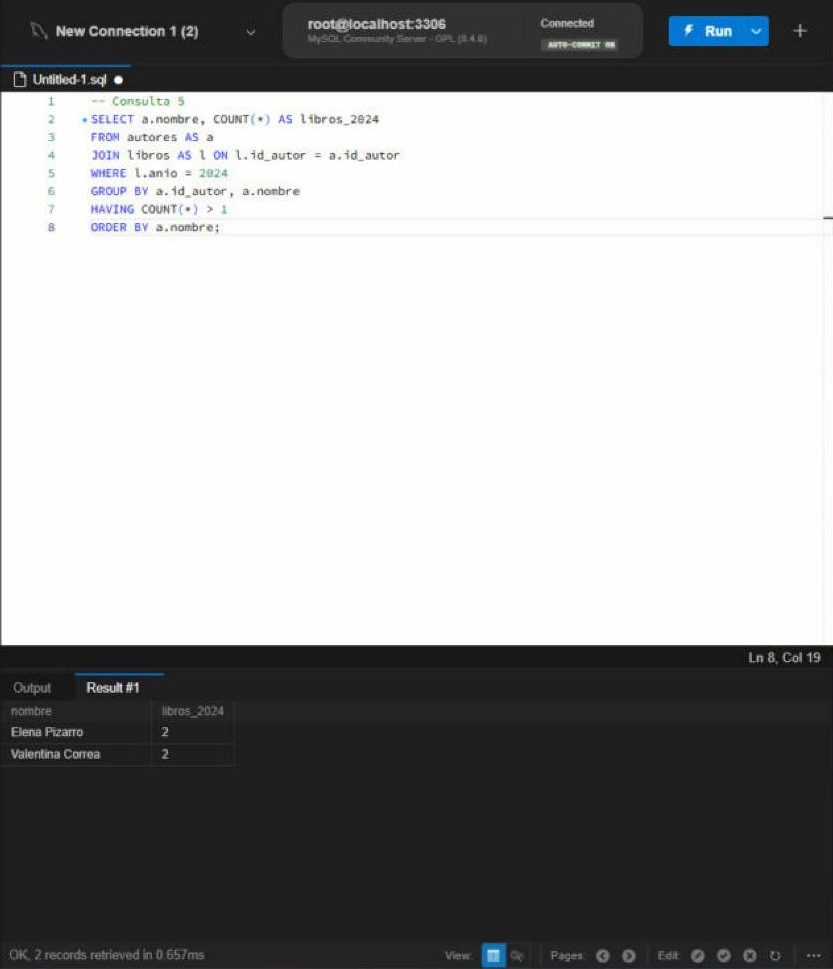
\includegraphics[width=0.72\textwidth]{imagenes/c05.jpg}
\caption{Resultado de la consulta 5}
\end{figure}

\clearpage
\section*{Consulta 6}
\begin{figure}[H]
\begin{lstlisting}
-- Consulta 6
SELECT titulo, ejemplares_vendidos
FROM libros
WHERE anio = 2024 AND ejemplares_vendidos > 2000
ORDER BY ejemplares_vendidos DESC
LIMIT 3;
\end{lstlisting}
\centering
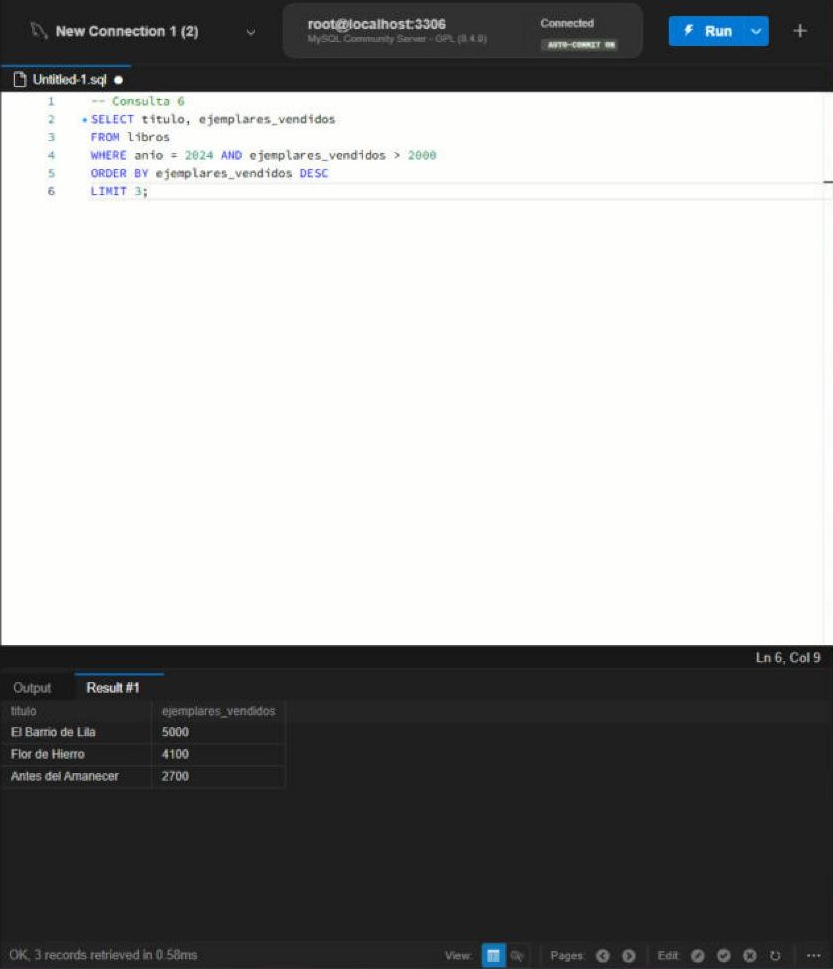
\includegraphics[width=0.72\textwidth]{imagenes/c06.jpg}
\caption{Resultado de la consulta 6}
\end{figure}

\clearpage
\section*{Consulta 7}
\begin{figure}[H]
\begin{lstlisting}
-- Workbench viene con safe updates activado y no deja hacer el DELETE ni el UPDATE filtrando por titulo
SET SQL_SAFE_UPDATES = 0;

-- Consulta 7
INSERT INTO libros (id_autor, titulo, paginas, ejemplares_vendidos, anio)
VALUES (3, 'Papel Mojado', 260, 50, 2024);
\end{lstlisting}
\centering
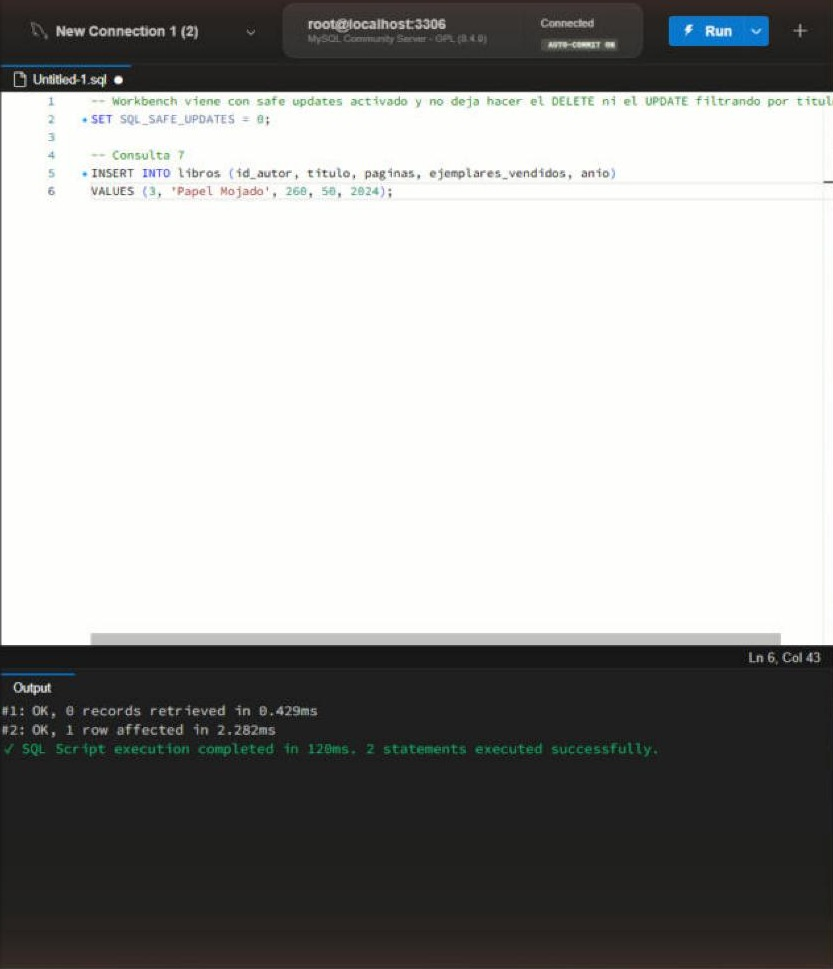
\includegraphics[width=0.72\textwidth]{imagenes/c07.jpg}
\caption{INSERT de Papel Mojado}
\end{figure}

\begin{figure}[H]
\begin{lstlisting}
SELECT * FROM libros WHERE titulo = 'Papel Mojado';
\end{lstlisting}
\centering
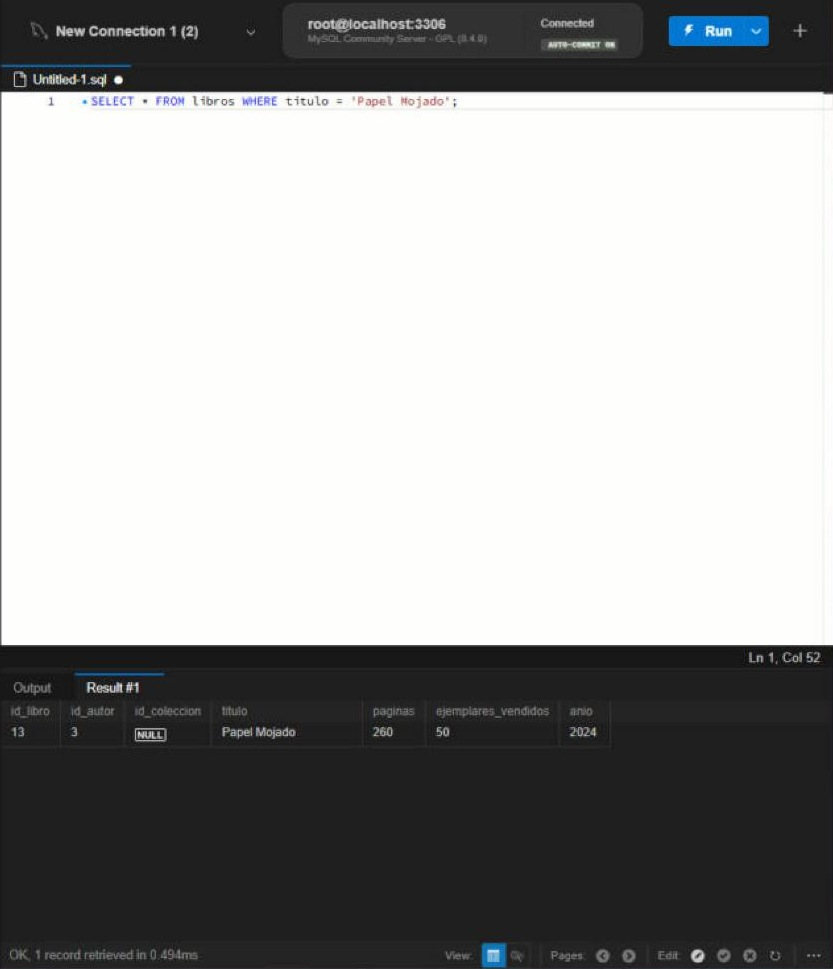
\includegraphics[width=0.72\textwidth]{imagenes/c08.jpg}
\caption{SELECT antes del DELETE}
\end{figure}

\begin{figure}[H]
\begin{lstlisting}
DELETE FROM libros WHERE titulo = 'Papel Mojado';
\end{lstlisting}
\centering
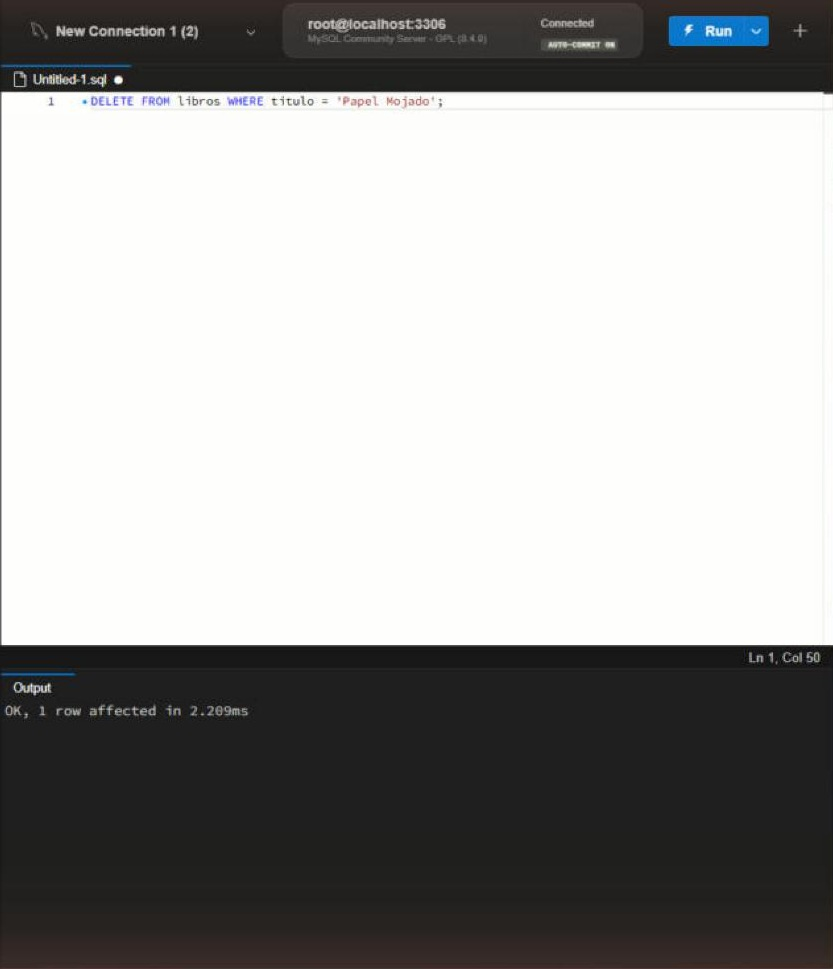
\includegraphics[width=0.72\textwidth]{imagenes/c09.jpg}
\caption{DELETE filtrando por título}
\end{figure}

\begin{figure}[H]
\begin{lstlisting}
SELECT * FROM libros WHERE titulo = 'Papel Mojado';
\end{lstlisting}
\centering
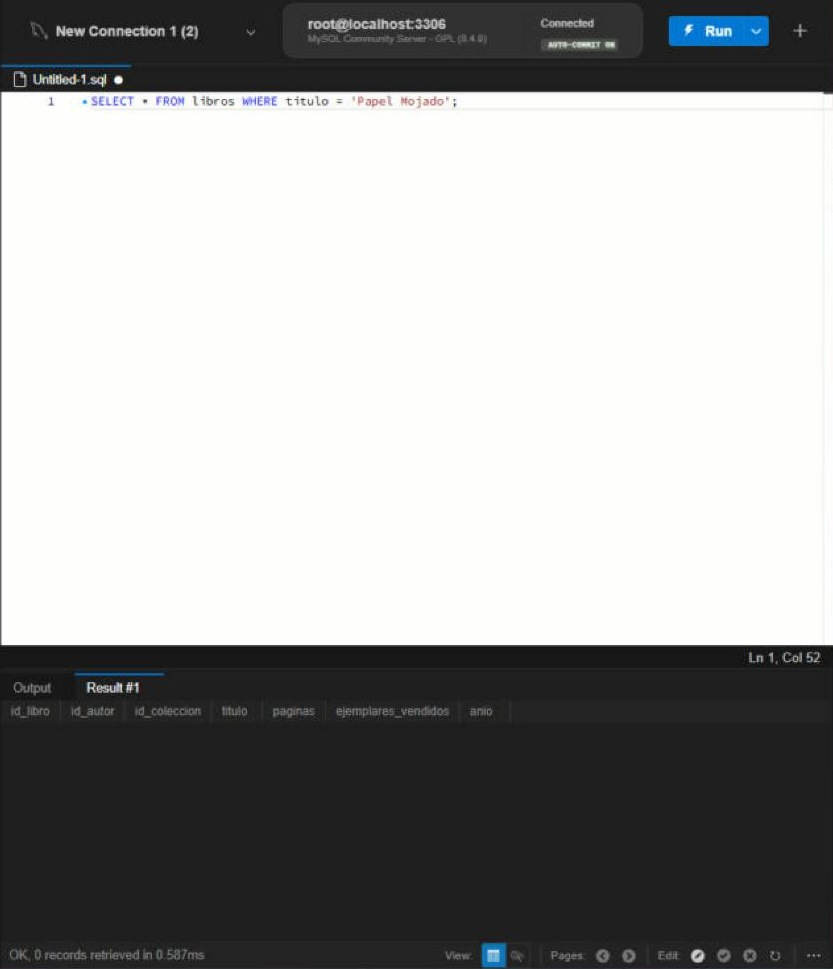
\includegraphics[width=0.72\textwidth]{imagenes/c10.jpg}
\caption{SELECT después del DELETE}
\end{figure}

\clearpage
\section*{Consulta 8}
\begin{figure}[H]
\begin{lstlisting}
-- Consulta 8
SELECT titulo, ejemplares_vendidos FROM libros WHERE titulo = 'Cielo de Enero';
\end{lstlisting}
\centering
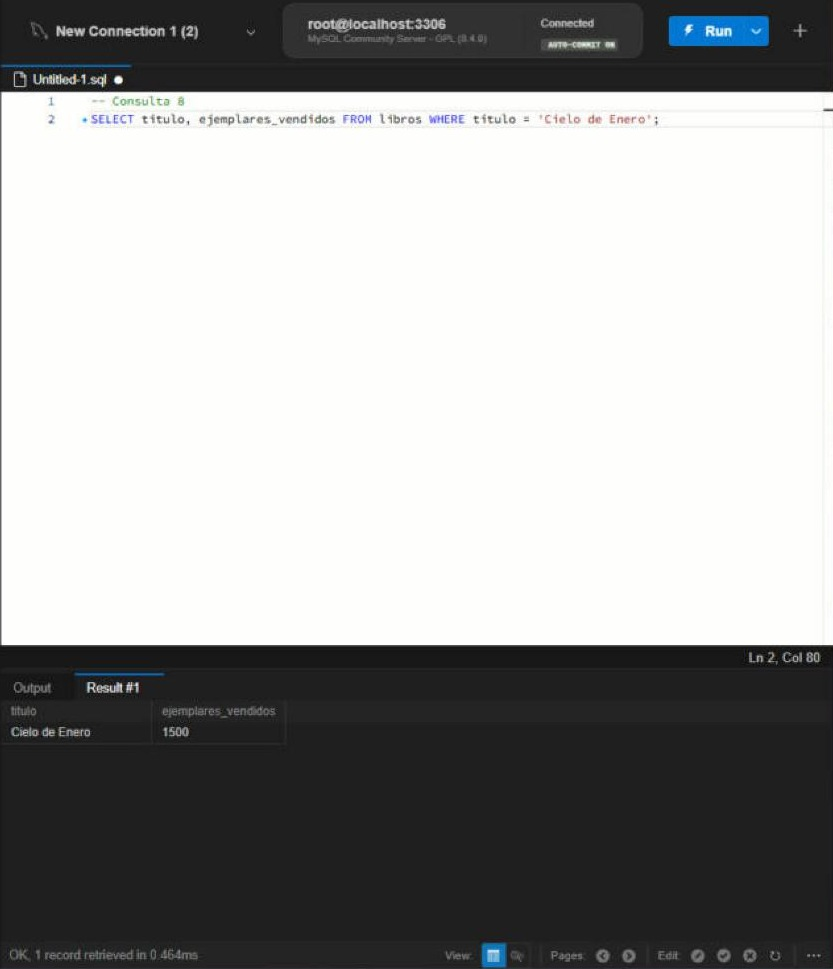
\includegraphics[width=0.72\textwidth]{imagenes/c11.jpg}
\caption{SELECT previo al UPDATE}
\end{figure}

\begin{figure}[H]
\begin{lstlisting}
UPDATE libros
SET ejemplares_vendidos = ejemplares_vendidos + 100
WHERE titulo = 'Cielo de Enero';
\end{lstlisting}
\centering
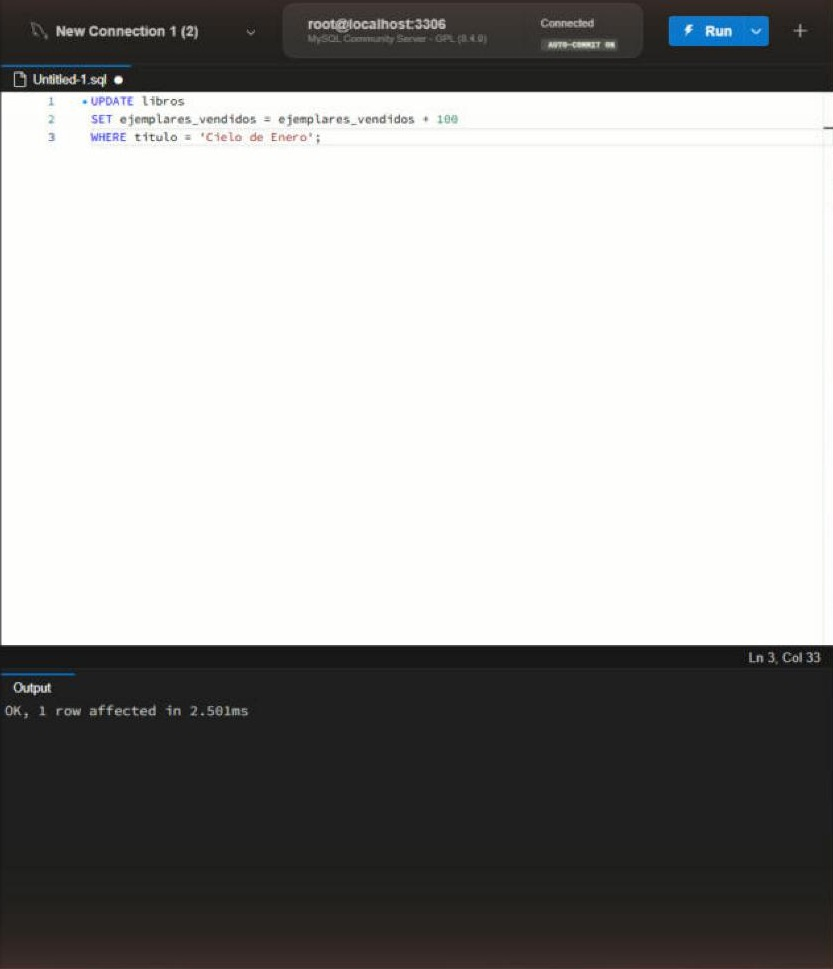
\includegraphics[width=0.72\textwidth]{imagenes/c12.jpg}
\caption{UPDATE de Cielo de Enero}
\end{figure}

\begin{figure}[H]
\begin{lstlisting}
SELECT titulo, ejemplares_vendidos FROM libros WHERE titulo = 'Cielo de Enero';
\end{lstlisting}
\centering
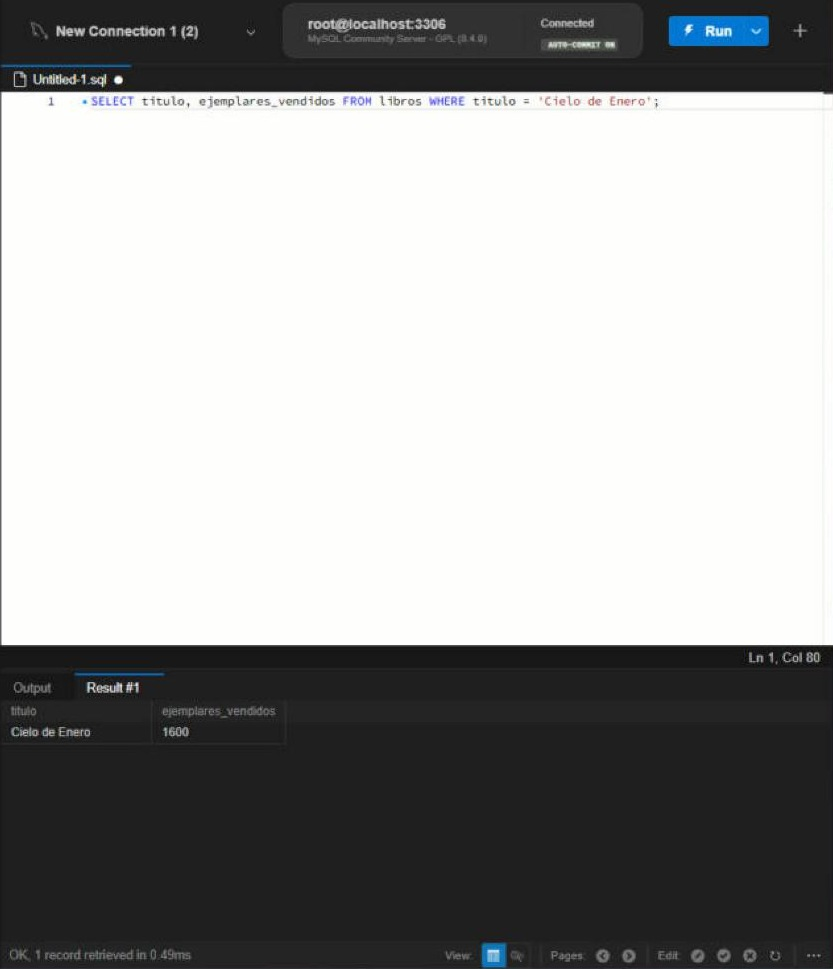
\includegraphics[width=0.72\textwidth]{imagenes/c13.jpg}
\caption{SELECT posterior al UPDATE}
\end{figure}

\clearpage
\section*{Consulta 9}
\begin{figure}[H]
\begin{lstlisting}
-- Consulta 9
INSERT INTO colecciones (titulo, fecha_publicacion) VALUES
    ('Narrativa del Sur', '2022-04-23'),
    ('Pensamiento y Verso', '2022-09-10'),
    ('Pequeños Lectores', '2023-03-27');

UPDATE libros SET id_coleccion = 1 WHERE id_autor = 1 OR id_autor = 5;
UPDATE libros SET id_coleccion = 2 WHERE id_autor = 2 OR id_autor = 3;
UPDATE libros SET id_coleccion = 3 WHERE id_autor = 4;
\end{lstlisting}
\centering
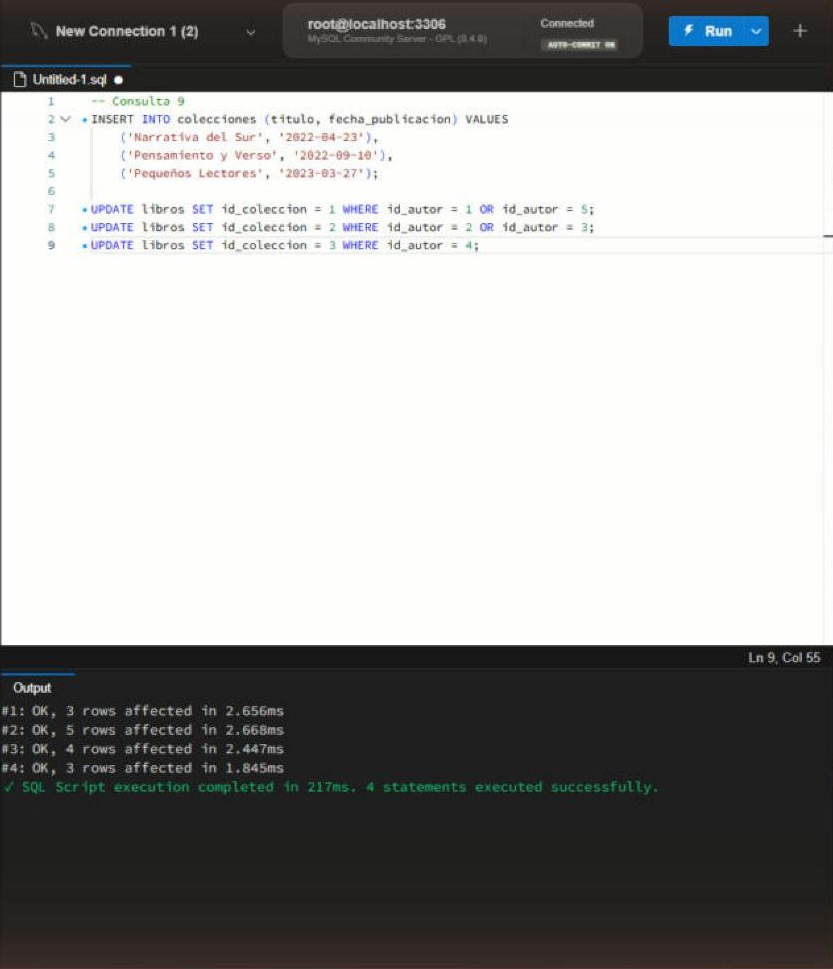
\includegraphics[width=0.72\textwidth]{imagenes/c14.jpg}
\caption{Carga de colecciones y asignación de los libros}
\end{figure}

\begin{figure}[H]
\begin{lstlisting}
SELECT l.titulo AS libro, c.titulo AS coleccion, c.fecha_publicacion
FROM libros AS l
JOIN colecciones AS c ON l.id_coleccion = c.id_coleccion
ORDER BY c.fecha_publicacion, l.titulo;
\end{lstlisting}
\centering
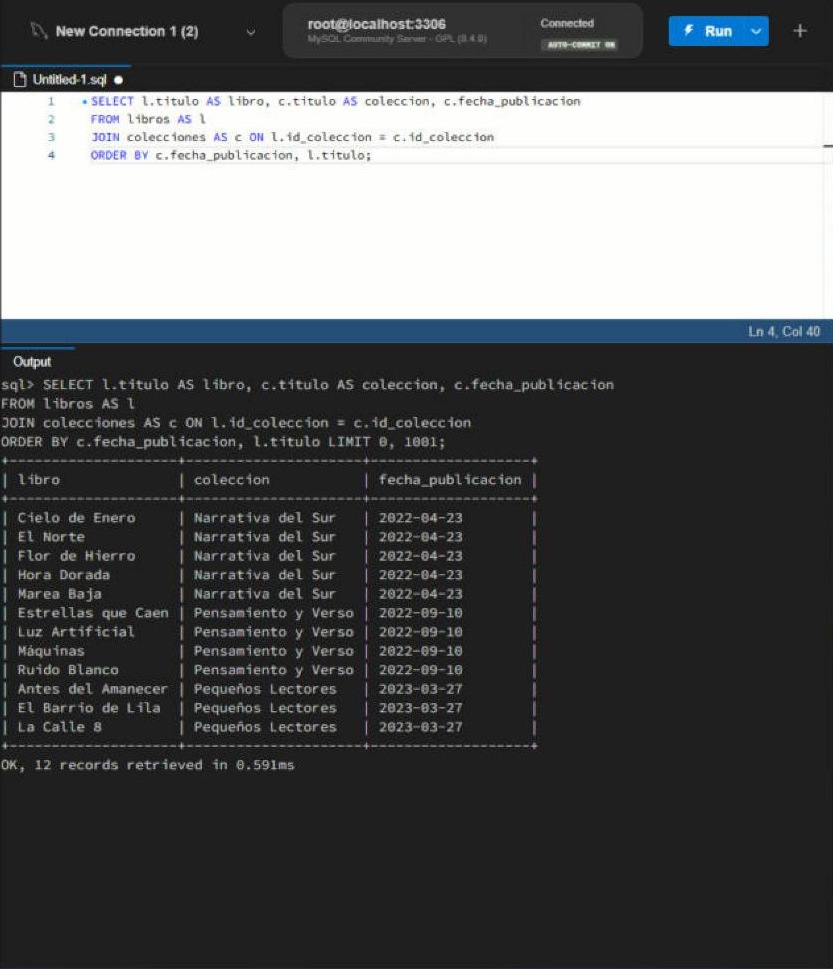
\includegraphics[width=0.72\textwidth]{imagenes/c15.jpg}
\caption{Libros con su colección y fecha de publicación}
\end{figure}

\clearpage
\section*{Consulta 10}
\begin{figure}[H]
\begin{lstlisting}
-- Consulta 10
INSERT INTO pagos (id_autor, fecha_pago, monto) VALUES
    (1, '2026-03-31', 850000.00),
    (4, '2026-04-15', 1250000.00),
    (1, '2026-09-30', 620500.50),
    (5, '2026-10-05', 980000.00);
\end{lstlisting}
\centering
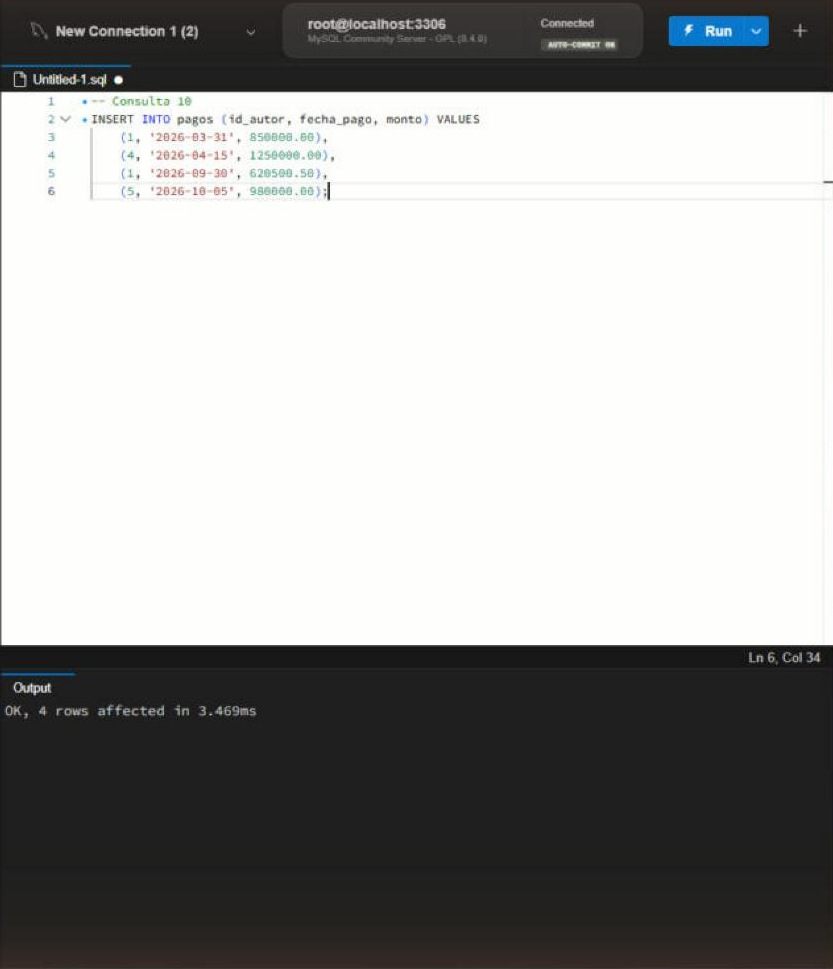
\includegraphics[width=0.72\textwidth]{imagenes/c16.jpg}
\caption{Carga de pagos}
\end{figure}

\begin{figure}[H]
\begin{lstlisting}
SELECT a.nombre, p.fecha_pago, p.monto
FROM pagos AS p
JOIN autores AS a ON p.id_autor = a.id_autor
ORDER BY p.fecha_pago;
\end{lstlisting}
\centering
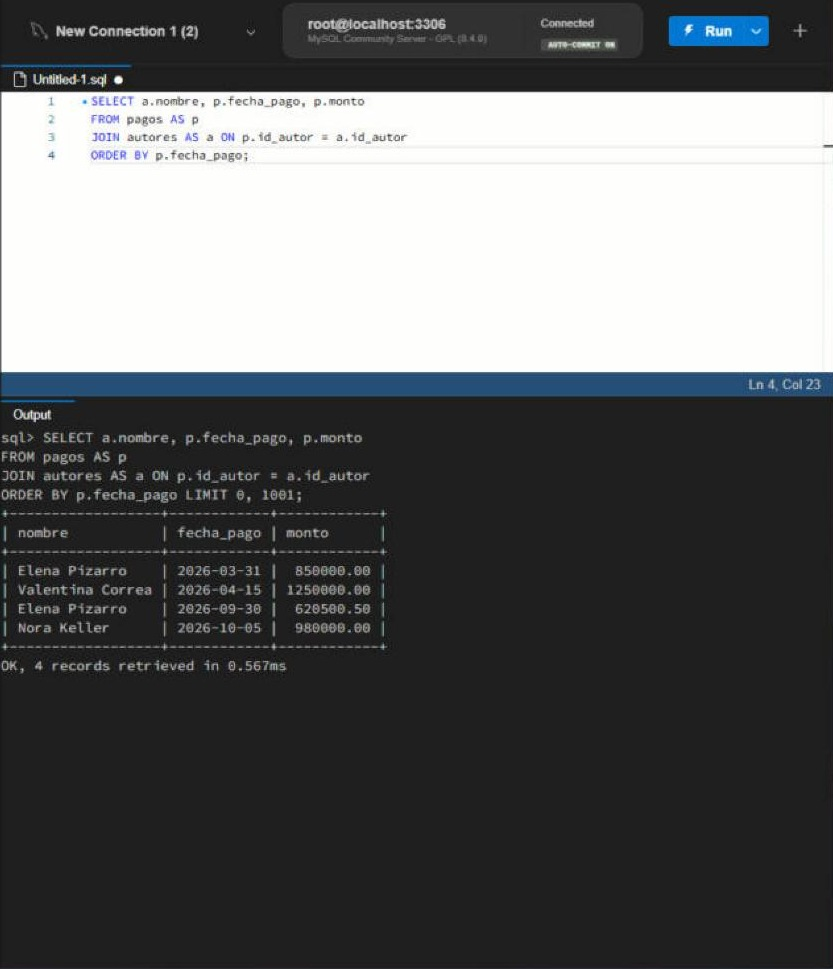
\includegraphics[width=0.72\textwidth]{imagenes/c17.jpg}
\caption{Pagos hechos a los autores}
\end{figure}

\begin{figure}[H]
\begin{lstlisting}
SELECT a.nombre, SUM(p.monto) AS total_pagado
FROM pagos AS p
JOIN autores AS a ON p.id_autor = a.id_autor
GROUP BY a.id_autor, a.nombre
ORDER BY a.nombre;
\end{lstlisting}
\centering
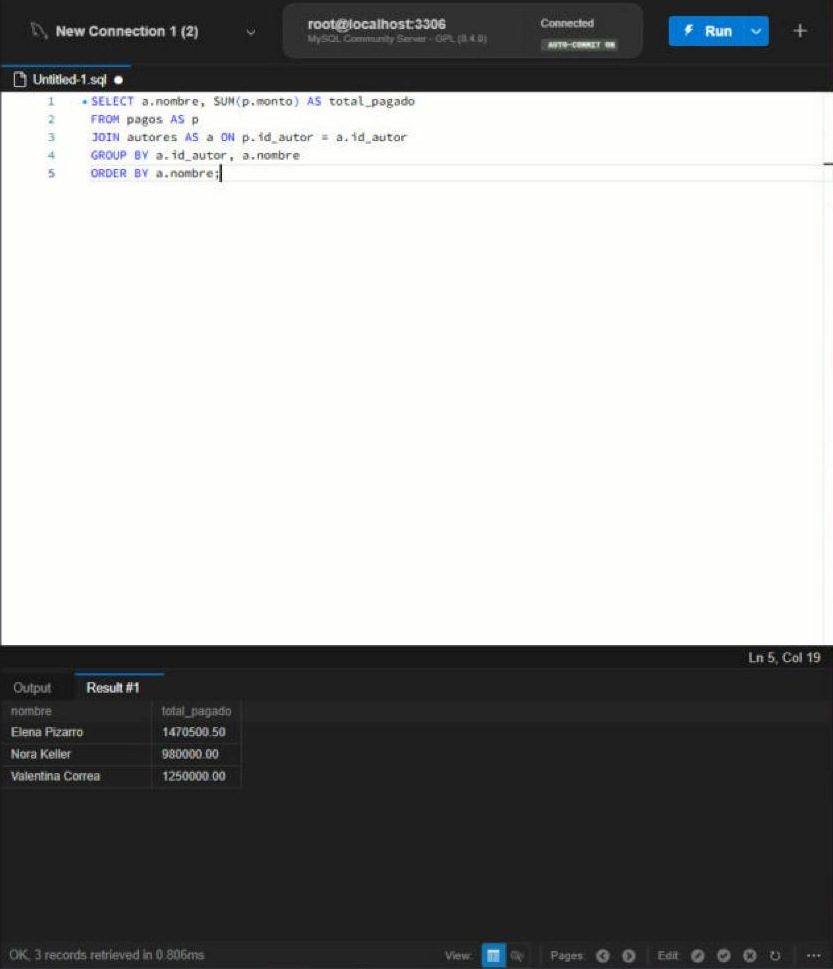
\includegraphics[width=0.72\textwidth]{imagenes/c18.jpg}
\caption{Total pagado a cada autor}
\end{figure}

\end{document}
